\documentclass{beamer}

\usepackage{physics}
\usepackage{hyperref}
\usepackage{url}

\newenvironment{itemframe}[1]{\begin{frame}{#1}\begin{itemize}}   {\end{itemize}\end{frame}}

% Changes style of actual slides
\usetheme{Dresden}
% Changes color of slides
\usecolortheme{spruce}
% removes controls at bottom right side
\usenavigationsymbolstemplate{}

% for figures
\graphicspath{ {./figs/} }

\title{The Carnot Engine}
\author{Michael Cardiff}
% \logo{\large \LaTeX{}}
\subtitle{PHYS 163a \\ 09/02 Prep Work}

\begin{document}

\begin{frame}
  \titlepage
\end{frame}

\section{What is Carnot's Engine?}
\begin{frame}{Kardar's Definition}
  \begin{center}
    \textit{A Carnot Engine is any engine that is \underline{reversible}, runs in a \underline{cycle}, with all of its \underline{heat exchanges} taking place at temperature $T_H$ and a sink temperature $T_C$}
  \end{center}
  We should break this down a bit
\end{frame}

\begin{frame}{Reversiblity}
  \begin{columns}
    \begin{column}{0.5\textwidth}
      \begin{itemize}
      \item Reversing a process = Going backward in time
      \item A reversible process can be run backward in time by swapping input and output
      \item For Carnot's engine, this means swapping $T_C$ with $T_H$ and vice versa
      \item Reversibility implies an Equilibrium
      \end{itemize}
    \end{column}
    \begin{column}{0.5\textwidth}
      \begin{figure}[H]
        \centering
        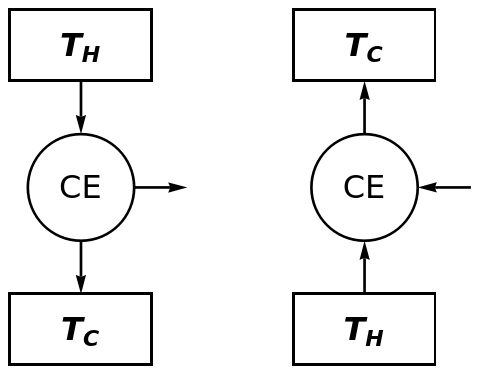
\includegraphics[width=5.0cm]{carnot.png}
        \caption{Carnot Engine and its reversal}
      \end{figure}
    \end{column}
  \end{columns}
  
\end{frame}

\begin{frame}{The Carnot Cycle}
    \begin{columns}
    \begin{column}{0.5\textwidth}
      \begin{itemize}
      \item Heat must be exchanged between two isotherms, at temperatures $T_H$ and $T_C$
      \item The Isotherms are then connected by \textit{adiabats} in which no heat is exchanged, this allows the cycle to close
      \item In The figure, the red lines are isoterms, and the blue are adiabats
      \end{itemize}
    \end{column}
    \begin{column}{0.5\textwidth}
      \begin{figure}[H]
        \centering
        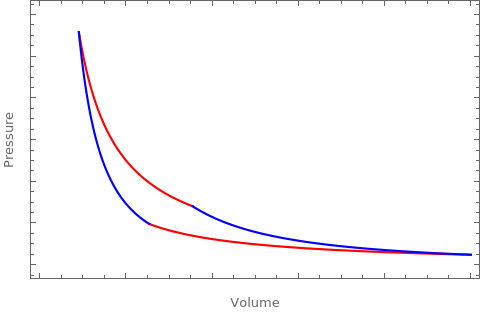
\includegraphics[width=5.0cm]{carnotcycle.png}
        \caption{Carnot Cycle Example}
      \end{figure}
    \end{column}
  \end{columns}  
\end{frame}

\begin{frame}{Heat Exchanging}
  \begin{itemize}
  \item While there is not net change during the adiabatic processes, there is during the isothermal processes
  \item Work is given off\footnote{In an engine} in order to actually cool the medium from $T_H$ to $T_C$
  \item Work is absorbed\footnote{In a refrigerator} into the system in order to cool $T_H$ down to $T_C$
  \end{itemize}
\end{frame}

\section{Engine Efficiency}
\begin{frame}{Engine Efficiency}
  The efficiency of an engine is the ratio of the work done (the output of the engine) to the heat absorbed. Mathematically:
  \begin{equation}
    \eta=\frac{W}{Q_H}
  \end{equation}
  Where $W$ is your engine output, and $Q_H$ is the heat absorbed from the heat source $T_H$.
\end{frame}

\section{The Universality of the Efficiency}
\begin{frame}{The Engine Medium Does not Matter}
  The efficiency of a carnot engine can be made without reference to a Carnot Cycle, which is dependent on a specific medium. We get that the entropy change (from section 1.6) will be 0. We then get:
  \begin{equation}
    0=-\frac{\abs{Q_H}}{T_C}+\frac{\abs{Q_C}}{T_H}
    \implies\frac{\abs{Q_C}}{\abs{Q_H}}=\frac{T_C}{T_H}
  \end{equation}
\end{frame}

\begin{frame}{The Engine Medium Does not Matter}
  This gives a relationship between $Q_H$ and $Q_C$, giving an efficiency for the Carnot engine without reference to the driving system:
  \begin{equation}
    \eta=\frac{W}{\abs{Q_H}}=1-\frac{\abs{Q_C}}{\abs{Q_H}}
    =\boxed{1-\frac{T_C}{T_H}}
  \end{equation}
\end{frame}

\section{The Carnot Engine is the Most Efficient}
\begin{frame}{The Carnot Engine is the Most Efficient Engine}
  \begin{itemize}
  \item Say we have another engine, which I claim is more efficient than the Carnot engine.
  \item Use this engine to run the Carnot engine as a refrigerator.
  \item The same work is produced by both engines, since they are effectively running each other.
  \end{itemize}
\end{frame}

\begin{frame}{The Carnot Engine is the Most Efficient}
  \begin{itemize}
    \item The net heat transfer must be positive
  \item The heat transferred is equal to $Q_H-Q_H'$, which we said was positive
    \begin{equation}
      Q_H-Q_H'>0\implies Q_H>Q_H'
    \end{equation}
  \item So when we flip this over to calculate the efficiency, we find:
    \begin{equation}
      \frac{W}{Q_H}<\frac{W}{Q_H'}\implies \eta_{c}>\eta_{other}
    \end{equation}
  \item So my claim that my engine is more efficient than the Carnot engine is wrong.
  \end{itemize}
\end{frame}
\end{document}